% Beamer slide template prepared by Tom Clark <tom.clark@op.ac.nz>
% Otago Polytechnic
% Dec 2012

\documentclass[10pt]{beamer}
\usetheme{Dunedin}
\usepackage{graphicx}
\usepackage{fancyvrb}

\newcommand\codeHighlight[1]{\textcolor[rgb]{1,0,0}{\textbf{#1}}}

\title{The Iterator Pattern}

\author[IN608]{Intermediate Application Development}
\institute[Otago Polytechnic]{
  Otago Polytechnic \\
  Dunedin, New Zealand \\
  Kaiako: Tom Clark
}
\date{}
\begin{document}

%----------- titlepage ----------------------------------------------%
\begin{frame}[plain]
  \titlepage
\end{frame}

%----------- slide --------------------------------------------------%
\begin{frame}[fragile]
  \frametitle{Introduction}
  
  We do this all the time:
  \begin{Verbatim}[commandchars=\\\{\}]
  
  for thing in \codeHighlight{aggregate}:
      do_stuff_with(thing)
  
  \end{Verbatim}
  
  \begin{enumerate}
    \item What kind of objects can do this?
    \item How does this work, anyway?     
  \end{enumerate}  
\end{frame}

%----------- slide --------------------------------------------------%
\begin{frame}
  \frametitle{Iterables}
  
  Objects that can be used in \texttt{for} loops like this are called \emph{Interables}.
  This means that they are capable of supplying \emph{Iterators}. In other words,
  they implement the Iterator Pattern.
  
  \vspace{5mm}
  ``Provide a way to access the elements of an aggregate object sequentially without exposing 
  its underlying implementation.'' \\
  (\emph{GoF})
  
  \vspace{5mm}
  This pattern is so fundamental that it is supported in the core Python language. Many common objects 
  implement Iterator, and it is easy to make your own objects that support it too.  

  
\end{frame}

%----------- slide --------------------------------------------------%
\begin{frame}
  \frametitle{Examples}
  
  \begin{itemize}
    \item Lists
    \item Dictionaries
    \item Sets
    \item Files
    \item Database query results
  \end{itemize}  
       
\end{frame}

%----------- slide --------------------------------------------------%
\begin{frame}[fragile]
  \frametitle{Iterators in Action}

  \begin{verbatim}
  ls = [1, 2, 3]  # ls is an Iterable
  itr = iter(ls)  # itr is a list Iterator
  next(itr) # returns 1
  next(itr) # returns 2
  next(itr) # returns 3
  next(itr) # raises a StopIteration exception
  
  \end{verbatim}
 \end{frame} 

%----------- slide --------------------------------------------------%
\begin{frame}[fragile]
  \frametitle{Iterators in Action}

  These loops are equivalent.
  \begin{verbatim}

  ls = [1, 2, 3]
  
  for i in ls:
      print(i)
        
  itr = iter(ls) 
  while True:
      try:
          print(next(itr))
      except StopIteration:
          break    
  
  
  \end{verbatim}
 \end{frame} 


%----------- slide --------------------------------------------------%
\begin{frame}
  \frametitle{Structural Diagram} 
  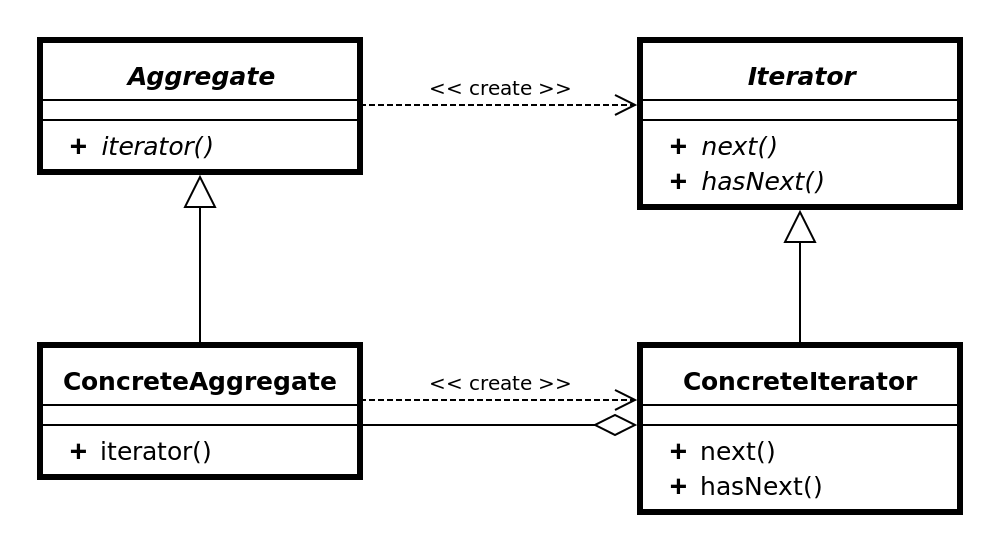
\includegraphics[width=8cm]{iterator.png}
  \end{frame}
  

%----------- slide --------------------------------------------------%
\begin{frame}
  \frametitle{Why a Seperate Iterator?}
  There is an important reason why an Iterable like a list
  produces a seperate Iterator. We may want to obtain two 
  Iterators from the same list. We expect that each iterator produces
  the list values independently.
  
  \vspace{5mm}
  A File object is a notable exception to this. It is its own Iterator.
  This is because we expect to be able to read from an open File up to 
  a point and then later resume reading from where we left off.
 \end{frame} 
 
%----------- slide --------------------------------------------------%
\begin{frame}[fragile]
  \frametitle{List vs File }

  \begin{verbatim}
  ls = [1, 2, 3]
  
  # these both print the same thing
  for i in ls:
      print(i)
      
  for i in ls:
      print(i)  
      
  with open('filename') as f: # f is an iterator
      for line in f:
          print(line)
          if line == '\n':
              break
      
      # this picks up reading where the loop above stopped
      for line in f:
          print(line)              
  \end{verbatim}
 \end{frame} 

 %----------- slide --------------------------------------------------%
\begin{frame}
  \frametitle{Programming Activity}
  
  \begin{enumerate}
    \item Pull the course materials repo.
    \item Create a new branch, \texttt{12-practical} in your practicals repo.
    \item Add a subdirectory,  \texttt{12-practical} and copy \texttt{11-practical.ipynb} from the class materials into it.
    \item Open a shell, cd to this directory, and run \texttt{jupyter notebook} to open the notebook. Complete the first two questions.
    \item We will discuss results in 20ish minutes.
  \end{enumerate}      
\end{frame}

%----------- slide --------------------------------------------------%
\begin{frame}[fragile]
  \frametitle{Make a Class Iterable}
  We make a class iterable by implementing the \texttt{\_\_iter\_\_} method.
  It must return an Iterator.
  
  \begin{Verbatim}[commandchars=\\\{\}]
  
  class Cattery:
  
    def __init__(self, cats):
        self._cats = set(cats)
        
    \codeHighlight{def __iter__(self):}
        \codeHighlight{return iter(self._cats)  }
           
  \end{Verbatim}
       
\end{frame} 



%----------- slide --------------------------------------------------%
\begin{frame}[fragile]
  \frametitle{Make an Iterator}
  Since an Iterable needs to provide an Iterator, sometimes
  we make our own Iterator class. To make a class an Iterator,
  implement a \texttt{\_\_next\_\_} method.
  
  \begin{Verbatim}[commandchars=\\\{\}]
        
   class SkipperIterator:
  
    def __init__(self, lst):
        self._lst = lst
        self._next_index = 0
        
    \codeHighlight{def __next__(self):}
        try:
            result = self._lst[self._next_index]
            self._next_index += 2
            return result
        except IndexError:
            raise StopIteration       
           
  \end{Verbatim}
       
\end{frame} 

%----------- slide --------------------------------------------------%
\begin{frame}[fragile]
  \frametitle{Using the Iterator}
  
  Now we just need an Iterable that uses our Iterator
    
  \begin{Verbatim}[commandchars=\\\{\}]
  
  class Skipper:  
  
    def __init__(self, lst):
        self._lst = list(lst)
        
    def __iter__(self):
        return SkipperIterator(self._lst)
        
    \end{Verbatim}
  Notice how the Iterable and the Iterator are tightly coupled. That's typical 
  of this pattern.     
\end{frame} 
\end{document}
